\documentclass[a4paper, twoside]{article}

\usepackage[ngerman]{babel}
\usepackage{mathtools, csquotes, graphicx}
\usepackage[margin=2.5cm]{geometry}

\setlength{\parindent}{0pt}
\setlength{\parskip}{1em}

\graphicspath{{./Grafiken/}}

\title{Formelsammlung---Numerische Methoden}
\author{Tim Hilt \and Emil Slomka}
\date{\today}

\begin{document}

\maketitle

\section{Lineare Gleichungssysteme}

Die unten beschriebenen Verfahren suchen Lösungen für die $x$-Werte. 

\subsection{Jacobi-Iteration}

\subsubsection{Jacobi-Iteration in Matrix-Vektor-Notation}

$\mathbf{L}$: Unterer Teil der Matrix

$\mathbf{D}$: Diagonale der Matrix

$\mathbf{U}$: Oberer Teil der Matrix

\[\mathbf{x}^{(k+1)} = -\mathbf{D}^{-1} (\mathbf{L} + \mathbf{U})\mathbf{x}^{(k)} + \mathbf{D}^{-1}\mathbf{b}\]

\textbf{Achtung}: Wenn bei der Jacobi-Iteration alle Startwerte $=0$ sind muss \textbf{Nur der zweite Term} $\mathbf{D}^{-1}\mathbf{b}$ betrachtet werden!!!

\subsubsection{Vorgehen}

\begin{enumerate}
\item Stelle einzelne Gleichungen auf
\item Auflösen nach den Variablen der jeweiligen Zeile
\item Links steht jetzt die Variable der nächsten Iteration, rechts stehen die vorhergehenden Werte.
\item Gleichungen ausrechnen
\end{enumerate}

\subsection{Gauss-Seidel-Iteration}

Die Gauss-Seidel-Iteration funktioniert genauso wie die Jacobi-Iteration, mit dem Unterschied, dass neu berechnete Werte direkt weiterverwendet werden.

\subsection{Konvergenz}

Die untenstehenden Kriterien stellen das Konvergenzkriterium für beide Iterationsverfahren (Jacobi genauso wie Gauss-Seidel) dar. Es gilt sowohl für das Jacobi- als auch für das Gauss-Seidel-Verfahren und für beliebige Startwerte.

\subsubsection{Diagonaldominanz}

Eine Matrix ist dann diagonaldominant, wenn in allen Zeilen der Betrag des Diagonalelements der Matrix größer ist als die Summe des Betrages der restlichen Elemente.

Wenn die Matrix \(A\) diagonaldominant ist ist eine Konvergenz der Iterationsverfahren garantiert. Ist sie nicht diagonaldominant, so ist die Konvergenz nicht garantiert (jedoch trotzdem nicht ausgeschlossen).

\[\sum_{j \neq k} |a_{ij}| < |a_{kk}| \ \text{für}\ k = 1, \ldots , n.\]

\subsubsection{Spektralradius}

\[\rho(\mathbf{A}) = \max_{j=1,\ldots,n} |\lambda_{j}| = \max(|-\mathbf{D}^{-1}(\mathbf{L} + \mathbf{U})|)\]

\(\Rightarrow\) Die Iteration konvergiert, wenn \(|\rho(\mathbf{A})| < 1\)

\(\Rightarrow\) Je kleiner der Spektralradius, desto schneller die Konvergenz


\section{Nicht-lineare Gleichungssysteme}

\subsection{Fixpunktiteration}

Gegeben ist ein nichtlineares Gleichungssystem (NGS), dessen Nullstellen es zu bestimmen gilt. Das gegebene NGS hat in unserem Fall nur eine einzelne Variable. Zur Berechnung der Nullstellen der Funktion \(f\) müssen wir die Funktion:

\begin{enumerate}
\item \(=0\) setzen
\item Nach \(x\) auflösen (auf der anderen Seite steht dann die Iterationsfunktion \(g(x)\))
\item Gegeben ist ein Startwert \(x^{(0)}\), der in \(g(x)\) eingesetzt wird um \(x^{(k+1)}\) zu berechnen
\end{enumerate}

Konvergiert die Fixpunktfunktion \(g\) gegen einen Fixpunkt \(x^{\star}\), dann ist dieser Fixpunkt eine Nullstelle von \(f\).

\subsection{Eigenschaften von Iterationsfunktionen}

\subsection{Konvergenz}

\subsubsection{Alternierende Konvergenz}

Wenn bei einer konvergenten Zahlenfolge der nachfolgende Wert \(x^{(k+1)}\) zwischen den beiden Vorgängerwerten \(x^{(k-1)}\) und \(x^{(k)}\) liegt, d.h.

\[x^{(k+1)} \leq x^{(k+1)} \leq x^{(k)},\quad k = 1, 2, \ldots\]

oder

\[x^{(k)} \leq x^{(k+1)} \leq x^{(k-1)},\quad k = 1, 2, \ldots\]

dann bezeichnet man die Konvergenz als \textbf{alternierend}.

\subsubsection{Monotone Konvergenz}

Bei einer konvergenten Zahlenfolge spricht man von \textbf{monoton fallender Konvergenz},
wenn die nachfolgenden Werte stets kleiner sind als die Vorgängerwerte

\[x^{(k+1)} \leq x^{(k)},\quad k = 1, 2, \ldots\]

und von \textbf{monoton wachsender Konvergenz}, wenn die nachfolgenden Werte stets
größer sind als die Vorgängerwerte

\[x^{(k+1)} \geq x^{(k)},\quad k = 1, 2, \ldots\]

\subsection{Konvergenz der Fixpunktiteration}

\subsection{Lipschitz}

\subsection{Fehlerabschätzung}

\subsubsection{A priori}

Bsp.: \enquote{Wie viele Iterationen benötigt man, um die Genauigkeit \(x\) zu erreichen?}

\enquote{Welche Genauigkeit erhält man nach \(k\) Iterationen?}

\subsubsection{A posteriori}

\section{Interpolation und Approximation}

\subsection{Newton-Tableau}

\clearpage

\subsection{Hermite-Tableau}

Das Hermite-Tableau stellt eine Generalisierung der Newton-Tableaus dar, mithilfe derer auch Eigenschaften der Ableitungen ins Interpolationspolynom aufgenommen werden können.

\paragraph{Beispiel}

Gegeben:

{\centering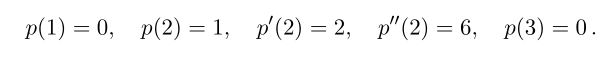
\includegraphics[width=.5\textwidth]{hermite_geg}\par}

Gesucht:

{\centering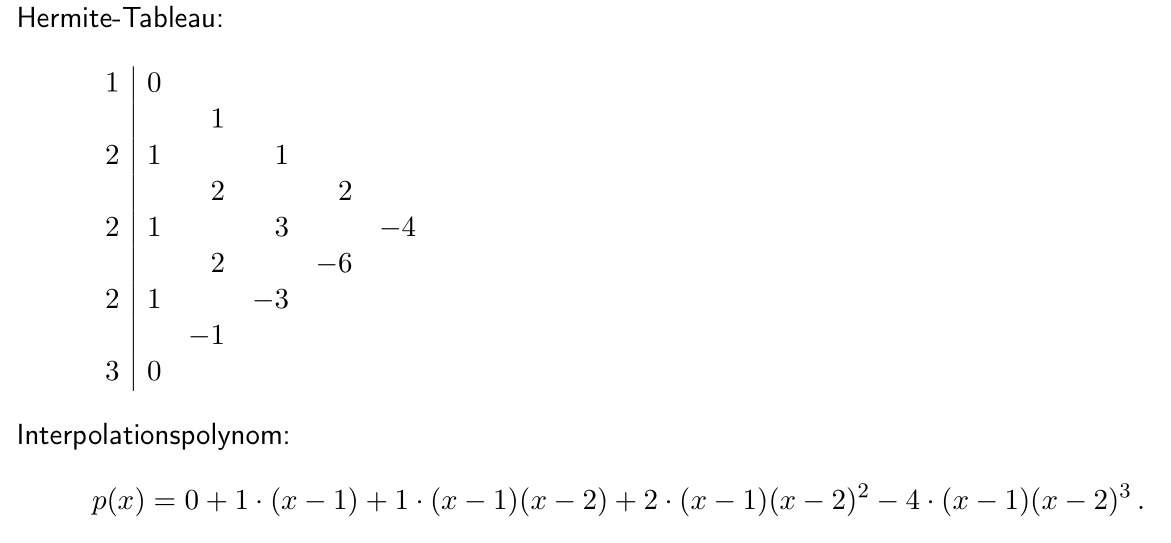
\includegraphics[width=.9\textwidth]{hermite_ges}\par}

\section{Numerische Integration}

\subsection{Trapezregel}

\[h = \frac{b-a}{n}\]

\[T(h) = h\left(\frac{1}{2}f(a) + f(a+h) + f(a+2h) + \ldots + f(a + (n-1)h) + \frac{1}{2}f(b)\right)\]

\[T(h) = h \cdot \left( \frac{1}{2} \cdot (f(a) + f(b)) + \sum_{k=1}^{n-1} f(a + k \cdot h)\right)\]

% \subsubsection{Summierte Trapezregel}

\subsection{Romberg-Verfahren}

\begin{align*}
  T(4)_{1} &&\\
  T(2)_{1} & \qquad\rightarrow T(2)_{2} = \frac{4}{3} \cdot T(2) - \frac{1}{3} \cdot T(4) &&\\
  T(1)_{1} & \qquad\rightarrow T(1)_{2} = \frac{4}{3} \cdot T(1) - \frac{1}{3} \cdot T(2) & \rightarrow T(1)_{3} = \frac{16}{15} \cdot T(1)_{2} - \frac{1}{15} \cdot T(2)_{2}
\end{align*}

\section{Optimierung}

\subsection{Gradientenverfahren}

\[\mathbf{x}^{(k+1)} = \mathbf{x}^{k} - t^{(k)} \cdot \nabla f\left(\mathbf{x}^{(k)}\right)\]

\section{Gewöhnliche Differenzialgleichungen}

\subsection{Eulerverfahren}

\[x'(t) = f(t, x(t)),\quad x(t_{0}) = x_{0},\quad t \in [t_{0}, t_{n}]\]

\begin{align*}
  \tilde{x}_{k+1} &= \tilde{x}_{k} + h \cdot f(t_{k}, \tilde{x}_{k})\\[1em]
  t_{k+1} &= t_{k} + h
\end{align*}

\subsubsection{Fehlerabschätzung / Toleranz}

\paragraph{Lokaler Fehler}

Benötigt:

\begin{itemize}
\item \(\tilde{x}^{(k+1)}\): Näherungswert nach einem Iterationsschritt mit Schrittweite \(h\)
\item \(\tilde{y}^{(k+1)}\): Näherungswert nach \textbf{zwei} Iterationsschritten mit Schrittweite \(h/2\)
\end{itemize}

\[e_{\text{lokal}} = |\tilde{x}^{(k+1)} - \tilde{y}^{(k+1)}|\]

\paragraph{Globaler Fehler}

\[e_{\text{global}} = \frac{|\tilde{x}^{(k+1)} - \tilde{y}^{(k+1)}|}{h}\]

\subsubsection{Optimale Schrittweite}

\[h_{\text{opt}} = \frac{\operatorname{tol} \cdot h}{|\tilde{x}^{(k+1)} - \tilde{y}^{(k+1)}|} \cdot h\]

\subsubsection{Schrittweitensteuerung}

Falls \(e_{\text{global}} > \operatorname{tol}\) setze \(h = h/2\)

Ansonsten berechne \(h_{\text{opt}}\) und setze \(h = h_{\text{opt}}\)

\end{document}